\documentclass[conference]{IEEEtran}
\IEEEoverridecommandlockouts

\usepackage{cite}
\usepackage{amsmath,amssymb,amsfonts}
\usepackage{algorithmic}
\usepackage{graphicx}
\usepackage{textcomp}
\usepackage{xcolor}
\usepackage{booktabs}
\usepackage{listings}

\lstset{
  basicstyle=\footnotesize\ttfamily,
  keywordstyle=\color{blue}\bfseries,
  commentstyle=\color{gray},
  stringstyle=\color{purple},
  breaklines=true,
  frame=single,
  numbers=none
}

\def\BibTeX{{\rm B\kern-.05em{\sc i\kern-.025em b}\kern-.08em
    T\kern-.1667em\lower.7ex\hbox{E}\kern-.125emX}}

\begin{document}

\title{Modeling, Simulation, and Optimal Control of an Underactuated Double Inverted Pendulum on a Cart System}

\author{
\IEEEauthorblockN{Tymur Omelianchuk}
\IEEEauthorblockA{\textit{Faculty of Applied Sciences} \\
\textit{Ukrainian Catholic University}\\
Lviv, Ukraine \\
t.omelianchuk.pn@ucu.edu.ua}
\and
\IEEEauthorblockN{Severyn Konoval}
\IEEEauthorblockA{\textit{Faculty of Applied Sciences} \\
\textit{Ukrainian Catholic University}\\
Lviv, Ukraine \\
s.konoval.pn@ucu.edu.ua}
\and
\IEEEauthorblockN{Oleksandr Oksentiuk}
\IEEEauthorblockA{\textit{Faculty of Applied Sciences} \\
\textit{Ukrainian Catholic University}\\
Lviv, Ukraine \\
oksentiuk.pn@ucu.edu.ua}
\and
\IEEEauthorblockN{Olesia Arlamovska}
\IEEEauthorblockA{\textit{Faculty of Applied Sciences} \\
\textit{Ukrainian Catholic University}\\
Lviv, Ukraine \\
arlamovska.pn@ucu.edu.ua}
\and
\IEEEauthorblockN{Ivan Shevtsov}
\IEEEauthorblockA{\textit{Project Mentor} \\
\textit{Staff Embedded Engineer, Samsung R\&D Institute Ukraine}\\
Lviv, Ukraine \\
}
}

\maketitle

\begin{abstract}
The inverted pendulum on a movable cart is an underactuated, open-loop unstable dynamical benchmark in modern control theory and robotics. Expanding the configuration from a single link to multiple links introduces strong nonlinear cross-coupling, severe sensitivity to external disturbances, and chaotic state-space dynamics. This paper presents an integrated engineering workflow for the modeling, simulation, and optimal control of both single and double inverted pendulum systems mounted on a motorized linear cart. Utilizing the Euler-Lagrange formalism, the full nonlinear equations of motion are derived, followed by local linearization around the upright equilibrium to construct state-space representations. After confirming full controllability via the Kalman rank criterion, continuous-time Linear-Quadratic Regulators (LQR) are synthesized by solving the Algebraic Riccati Equation for balancing. To address the narrow basin of attraction of linear regulators, an energy-based Lyapunov swing-up controller is developed for the single cart-pole system, while an energy-optimal Nonlinear Model Predictive Control (NMPC) scheme using CasADi and IPOPT is designed for offline swing-up trajectory generation of the double pendulum. The resulting hybrid control architectures are validated within 60~FPS interactive real-time simulators powered by 4th-order Runge-Kutta integration, and translated into an embedded C/C++ control routine suitable for microcontroller execution.
\end{abstract}

\begin{IEEEkeywords}
Underactuated systems, Double Inverted Pendulum, Euler-Lagrange dynamics, Linear-Quadratic Regulator (LQR), Nonlinear Model Predictive Control (NMPC), Energy Swing-Up, Embedded Control.
\end{IEEEkeywords}

\section{Introduction}
Underactuated mechanical systems---characterized by having fewer independent control inputs than degrees of freedom---serve as foundational testbeds for robotic manipulation, legged locomotion, and aerospace attitude control~\cite{ref_brunton, ref_den}. The classical inverted pendulum on a linear track is an iconic benchmark of this class~\cite{ref_astrom}. When an additional unactuated link is connected in series, forming a Double Inverted Pendulum (DIP), the dynamic complexity escalates substantially: inter-link centrifugal and Coriolis torques generate pronounced chaotic interactions, and infinitesimal disturbances precipitate system collapse without active closed-loop feedback~\cite{ref_spong, ref_den}.

Stabilizing both unactuated revolute joints in the upright vertical configuration necessitates generating horizontal inertial forces via cart motion alone~\cite{ref_task, ref_git}. Realizing a dependable and robust control framework entails:
\begin{enumerate}
    \item Formulating generalized coordinates and deriving nonlinear equations of motion via Euler-Lagrange mechanics~\cite{ref_task, ref_brunton}.
    \item Linearizing the equations around the unstable upright equilibrium and proving Kalman controllability~\cite{ref_task, ref_git}.
    \item Synthesizing optimal Linear-Quadratic Regulators (LQR) for local disturbance rejection and balancing~\cite{ref_brunton}.
    \item Designing an automated energy-pumping swing-up algorithm (Åström-Spong formulation) for single cart-pole setups~\cite{ref_astrom, ref_spong}.
    \item Formulating an energy-optimal Nonlinear Model Predictive Control (NMPC) strategy using CasADi and IPOPT for multi-body swing-up~\cite{ref_casadi, ref_git}.
    \item Engineering a modular, 60~FPS real-time simulation environment using 4th-order Runge-Kutta numerical integration with interactive physics-based mouse and keyboard perturbation interfaces~\cite{ref_git}.
    \item Implementing discrete-time embedded firmware routines suitable for low-power 32-bit microcontrollers~\cite{ref_git, ref_den}.
\end{enumerate}

This paper systematically documents the theoretical derivation, simulation implementation, and embedded realization of this control pipeline.

\section{Mathematical Modeling and Dynamics}

\subsection{Generalized Coordinates and Coordinate Frames}
The double inverted pendulum consists of a cart of mass $M$ traveling on a linear horizontal track with position $x(t)$, and two cascading links of masses $m_1, m_2$, lengths $L_1, L_2$, centers of mass located at distances $l_1, l_2$ from their respective pivot joints, and moments of inertia $I_1, I_2$ about their centers of mass~\cite{ref_git}. The generalized coordinate vector is:
\begin{equation}
q = \begin{bmatrix} x & \theta_1 & \theta_2 \end{bmatrix}^T
\end{equation}
where $\theta_1$ and $\theta_2$ denote the angular deflections of the first and second links with respect to the upward vertical axis ($\theta_i = 0$ corresponds to the perfectly upright position, and $\theta_i = \pi$ denotes downward suspension). The scalar control input $u(t)$ corresponds to the horizontal force applied to the cart.

\begin{figure}[htbp]
\centering
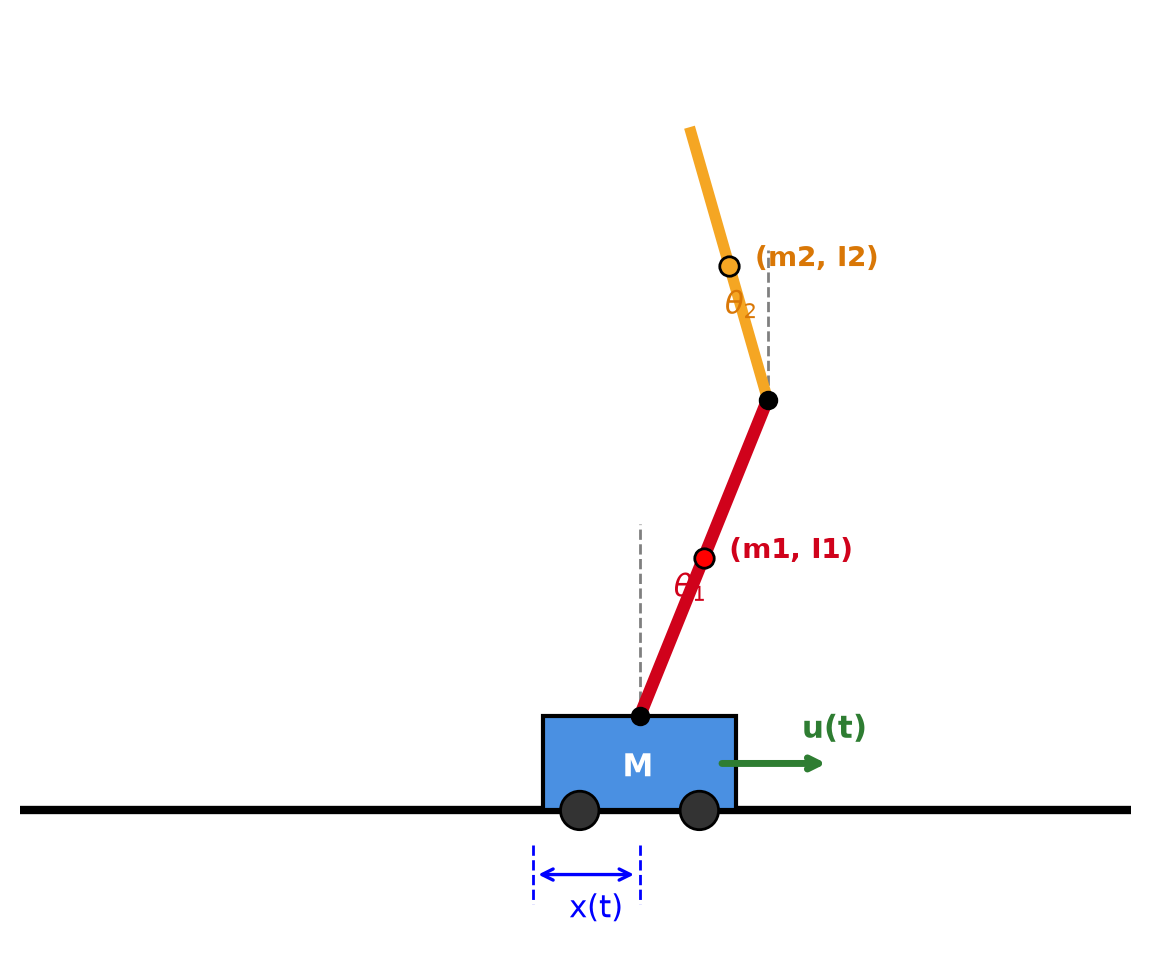
\includegraphics[width=0.85\columnwidth]{cart_pole_diagram.png}
\caption{Kinematic schematic and coordinate definitions for the underactuated double inverted pendulum on a motorized linear cart system.}
\label{fig:diagram}
\end{figure}

The Cartesian coordinates for the cart and link centers of mass shown in Fig.~\ref{fig:diagram} are formulated as:
\begin{align}
(x_c, y_c) &= (x, 0) \\
(x_{p1}, y_{p1}) &= (x + l_1 \sin\theta_1, l_1 \cos\theta_1) \\
(x_{p2}, y_{p2}) &= (x + L_1 \sin\theta_1 + l_2 \sin\theta_2, L_1 \cos\theta_1 + l_2 \cos\theta_2)
\end{align}

\subsection{Euler-Lagrange Equations of Motion}
The system dynamics are derived using the Lagrangian function $\mathcal{L} = T - V$ through the Euler-Lagrange equations:
\begin{equation}
\frac{d}{dt}\left(\frac{\partial \mathcal{L}}{\partial \dot{q}_i}\right) - \frac{\partial \mathcal{L}}{\partial q_i} = Q_i
\end{equation}
where $Q = [u - b_c\dot{x}, -b_1\dot{\theta}_1, -b_2\dot{\theta}_2]^T$ incorporates the control force $u$ and viscous friction dissipation terms: $b_c$ for the cart guide rail, and $b_1, b_2$ for the rotary bearings~\cite{ref_git}.

The total kinetic energy $T$ is the sum of translational and rotational components:
\begin{equation}
T = \frac{1}{2} M \dot{x}^2 + \sum_{k=1}^2 \left( \frac{1}{2} m_k (\dot{x}_{pk}^2 + \dot{y}_{pk}^2) + \frac{1}{2} I_k \dot{\theta}_k^2 \right)
\end{equation}

The potential energy $V$, with gravitational zero-reference at rail elevation ($y = 0$), is given by:
\begin{equation}
V = m_1 g l_1 \cos\theta_1 + m_2 g (L_1 \cos\theta_1 + l_2 \cos\theta_2)
\end{equation}
Note that under this upright convention, potential energy attains its global maximum at $\theta_1 = \theta_2 = 0$ and its minimum in the downward hanging configuration ($\theta_1 = \theta_2 = \pi$).

Carrying out the partial differentiations yields the standard second-order nonlinear matrix equation of motion~\cite{ref_brunton}:
\begin{equation}
M(q)\ddot{q} + C(q, \dot{q})\dot{q} + G(q) = B_u u
\label{eq:eom}
\end{equation}
where $M(q) \in \mathbb{R}^{3\times 3}$ is the positive-definite inertia matrix, $C(q, \dot{q}) \in \mathbb{R}^{3\times 3}$ accounts for Coriolis and centrifugal forces, $G(q) \in \mathbb{R}^3$ is the gravitational torque vector, and $B_u = [1, 0, 0]^T$.

For the baseline single cart-pole system ($M=1.0$~kg, $m=0.1$~kg, $L=1.0$~m, $l=0.5$~m, $I = \frac{1}{3}ml^2$), equation~\eqref{eq:eom} reduces to the classical coupled pair:
\begin{align}
(M + m)\ddot{x} + m l \ddot{\theta}\cos\theta - m l \dot{\theta}^2 \sin\theta + b_c \dot{x} &= u \\
m l \ddot{x}\cos\theta + (I + m l^2)\ddot{\theta} - m g l \sin\theta + b_p \dot{\theta} &= 0
\end{align}

\subsection{State-Space Linearization and Controllability}
To synthesize linear controllers, the nonlinear dynamics are linearized around the upright equilibrium:
\begin{equation}
q_0 = \begin{bmatrix} 0 & 0 & 0 \end{bmatrix}^T, \quad \dot{q}_0 = \begin{bmatrix} 0 & 0 & 0 \end{bmatrix}^T
\end{equation}
Applying small-angle approximations ($\sin\theta \approx \theta$, $\cos\theta \approx 1$), neglecting quadratic angular velocities ($\dot{\theta}^2 \approx 0$), and defining the state vector:
\begin{equation}
\mathbf{x} = \begin{bmatrix} x & \theta_1 & \theta_2 & \dot{x} & \dot{\theta}_1 & \dot{\theta}_2 \end{bmatrix}^T
\end{equation}
yields the continuous-time linear state-space model:
\begin{equation}
\dot{\mathbf{x}}(t) = A\mathbf{x}(t) + B u(t)
\label{eq:lin_ss}
\end{equation}

For the single cart-pole benchmark with state $\mathbf{x} = [x, \theta, \dot{x}, \dot{\theta}]^T$, defining $\mu = l(4M + m)$ with $I = \frac{1}{3}ml^2$, the system matrices simplify to:
\begin{equation}
A = \begin{bmatrix}
0 & 0 & 1 & 0 \\
0 & 0 & 0 & 1 \\
0 & -\frac{3mg}{4M + m} & 0 & 0 \\
0 & \frac{3(M + m)g}{l(4M + m)} & 0 & 0
\end{bmatrix}, \quad
B = \begin{bmatrix}
0 \\ 0 \\ \frac{4}{4M + m} \\ -\frac{3}{l(4M + m)}
\end{bmatrix}
\end{equation}

Evaluating the Kalman controllability rank criterion $\operatorname{rank}(\mathcal{C}) = \operatorname{rank}[B, AB, A^2B, A^3B] = 4$ for the single pendulum and $\operatorname{rank}(\mathcal{C}) = 6$ for the double pendulum verifies full controllability from the single scalar horizontal actuation input $u(t)$~\cite{ref_git}.

\section{Control System Design}

\subsection{Linear-Quadratic Regulator (LQR)}
The LQR optimal controller minimizes the infinite-horizon quadratic performance index:
\begin{equation}
J = \int_0^\infty \left( \mathbf{x}(t)^T Q \mathbf{x}(t) + u(t)^T R u(t) \right) dt
\end{equation}
where $Q \succeq 0$ penalizes state deviations and $R > 0$ penalizes actuator effort. The optimal state-feedback control law is:
\begin{equation}
u(t) = -K \mathbf{x}(t) = -R^{-1} B^T P \mathbf{x}(t)
\end{equation}
where $P$ is the unique positive-definite solution of the Continuous Algebraic Riccati Equation (CARE):
\begin{equation}
A^T P + P A - P B R^{-1} B^T P + Q = 0
\label{eq:care}
\end{equation}

For the single pendulum setup, setting state penalties $Q = \operatorname{diag}(q_x, q_\theta, q_v, q_\omega) = \operatorname{diag}(10.0, 140.0, 6.0, 20.0)$ and control weight $R = 0.1$ in \texttt{scipy.linalg.solve\_continuous\_are} yields the feedback gain vector:
\begin{equation}
u = k_\theta \theta + k_\omega \omega + k_x x + k_v v
\label{eq:lqr_formula}
\end{equation}
where $\omega = \dot{\theta}$ and $v = \dot{x}$. The resulting synthesized gains and operating limits are listed in Table~\ref{tab:gains}.

\begin{table}[htbp]
\caption{Synthesized Controller Gains and Physical Parameters (Single Cart-Pole Benchmark)}
\begin{center}
\begin{tabular}{llr}
\toprule
\textbf{Parameter} & \textbf{Physical Meaning / Role} & \textbf{Value} \\
\midrule
$M$        & Cart mass                         & 1.0~kg \\
$m$        & Pendulum rod mass                 & 0.1~kg \\
$L$        & Pendulum total length             & 1.0~m \\
$l$        & Pivot-to-CoM distance ($L/2$)     & 0.5~m \\
$k_\theta$ & Angular proportional restoring gain & 107.63~N/rad \\
$k_\omega$ & Angular velocity damping gain     & 30.74~N$\cdot$s/rad \\
$k_x$      & Cart position centering gain      & 10.00~N/m \\
$k_v$      & Cart linear velocity damper       & 15.73~N$\cdot$s/m \\
$u_{\max}$ & Actuator force saturation limit   & 19.80~N \\
$a_{\max}$ & Maximum allowable cart acceleration & 18.0~m/s$^2$ \\
$v_{\max}$ & Maximum linear velocity limit     & 3.2~m/s \\
$X_{\text{rail}}$ & Half-span rail track boundary & 2.2~m \\
\bottomrule
\end{tabular}
\label{tab:gains}
\end{center}
\end{table}

For the double inverted pendulum model in \texttt{hybrid\_mpc\_lqr}, the 6-state LQR uses diagonal weights $Q = \operatorname{diag}(15.0, 600.0, 800.0, 10.0, 45.0, 55.0)$ and $R = 0.08$, heavily prioritizing the verticality of both links ($\theta_1, \theta_2$) while softly regulating cart drift along the track.

\subsection{Lyapunov-Based Energy Swing-Up (Single Pendulum)}
Because linear models are valid only within a localized basin of attraction around the vertical apex, an energy swing-up controller is deployed to raise the pendulum from rest ($\theta = \pi$)~\cite{ref_astrom}.

Defining the total mechanical energy relative to the upright balance point:
\begin{equation}
E(\theta, \dot{\theta}) = \frac{1}{2} I \dot{\theta}^2 + m g l (\cos\theta - 1)
\end{equation}
the target energy is $E_0 = 0$. Differentiating with respect to time along trajectories of motion reveals:
\begin{equation}
\dot{E} = -m l \dot{\theta} \cos\theta \cdot a_{\text{cart}}
\end{equation}

Following the Åström-Spong formulation~\cite{ref_astrom, ref_spong}, the acceleration command is chosen proportional to the energy defect:
\begin{equation}
a_{\text{cart}} = k_E (E - E_0) \dot{\theta} \cos\theta + u_{\text{center}} + u_{\text{edge}}
\end{equation}
where $k_E = 75.0$, $u_{\text{center}} = -14x - 8v$ maintains the cart near rail center, and $u_{\text{edge}}$ provides soft virtual boundary repulsion. Once the pendulum approaches the linear capture zone ($|\theta| < 28^\circ \approx 0.49$~rad and $|\dot{\theta}| < 4.2$~rad/s), control authority switches to LQR balancing.

\subsection{Energy-Optimal NMPC Swing-Up (Double Pendulum)}
Due to complex nonlinear inter-link dynamics, single-degree-of-freedom Lyapunov energy pumping does not directly extend to double pendulums. We therefore employ a constrained Nonlinear Model Predictive Control (NMPC) formulation implemented using \texttt{do-mpc} with CasADi and the interior-point solver IPOPT~\cite{ref_casadi}.

The double inverted pendulum dynamics are expressed as a continuous Differential-Algebraic Equation (DAE) system. The optimal control problem maximizes total mechanical energy toward the upright target over a prediction horizon:
\begin{align}
\min_{\mathbf{u}, \mathbf{z}} \quad & \sum_{k=0}^{N-1} \left( E_{\text{kin}}(\mathbf{x}_k, \mathbf{z}_k) - E_{\text{pot}}(\mathbf{x}_k) \right) + \sum_{k=0}^{N-1} r_u (\Delta u_k)^2 \\
\text{s.t.} \quad & \mathbf{x}_{k+1} = F_{\text{colloc}}(\mathbf{x}_k, \mathbf{z}_k, u_k), \quad \mathbf{x}_0 = \mathbf{x}(t) \\
& g_{\text{DAE}}(\mathbf{x}_k, \mathbf{z}_k, u_k) = 0 \\
& -u_{\text{bound}} \le u_k \le u_{\text{bound}}
\end{align}
The optimization employs Radau orthogonal collocation (degree 3) with sampling time $t_{\text{step}} = 0.04$~s and horizon $N = 100$ steps (total lookahead window of $4.0$~s). Motor force bounds are restricted to $u_{\text{bound}} = 4.0$~N.

In our hybrid architecture (\texttt{hybrid\_mpc\_lqr}), this energy-optimal NMPC maneuver is computed offline and stored as an optimal feedforward policy $\mathbf{u}^*(t)$. During execution, an active supervisory Finite State Machine (FSM) initiates the precomputed MPC trajectory from downward rest ($\theta_1 = \theta_2 = \pi$), verifies continuous physical compliance without artificial state injection, and seamlessly executes handover to the 6-state LQR when both links enter the linear capture window ($|\theta_1| < 26^\circ, |\theta_2| < 26^\circ$).

\section{Simulation Engine and Tooling}

\subsection{Numerical Integration via Runge-Kutta 4}
Standard Euler integration exhibits significant artificial numerical dissipation and energy drift in stiff multi-body dynamics. Consequently, our physical simulation engines utilize an explicit 4th-order Runge-Kutta (RK4) integrator:
\begin{align}
k_1 &= f(\mathbf{x}_t, u) \\
k_2 &= f(\mathbf{x}_t + \tfrac{\Delta t}{2} k_1, u) \\
k_3 &= f(\mathbf{x}_t + \tfrac{\Delta t}{2} k_2, u) \\
k_4 &= f(\mathbf{x}_t + \Delta t k_3, u) \\
\mathbf{x}_{t+\Delta t} &= \mathbf{x}_t + \tfrac{\Delta t}{6}(k_1 + 2k_2 + 2k_3 + k_4)
\end{align}
Running at 60~FPS graphical update frequency ($\Delta t_{\text{frame}} \approx 16.67$~ms), each iteration executes 8 internal micro-steps ($\Delta t_{\text{sim}} \approx 2.08$~ms), maintaining numerical stability under rapid actuator reversals.

\subsection{Interactive Pygame Simulator}
The Pygame environment (\texttt{sim\_pygame.py}, Fig.~\ref{fig:pygame}) provides interactive manipulation: users can click and drag the cart or the pendulum bob via a virtual spring-damper coupling ($k_{\text{drag}} = 700$~N/m, $d_{\text{drag}} = 65$~N$\cdot$s/m), exciting realistic D'Alembert inertial reactions. On-screen sliders permit real-time retuning of $k_\theta, k_\omega, k_x, k_v$, and dynamic actuator saturation limits ($a_{\max}, v_{\max}$). An integrated oscilloscope renders live angular trajectory histories alongside target stability corridors.

\begin{figure}[htbp]
\centering
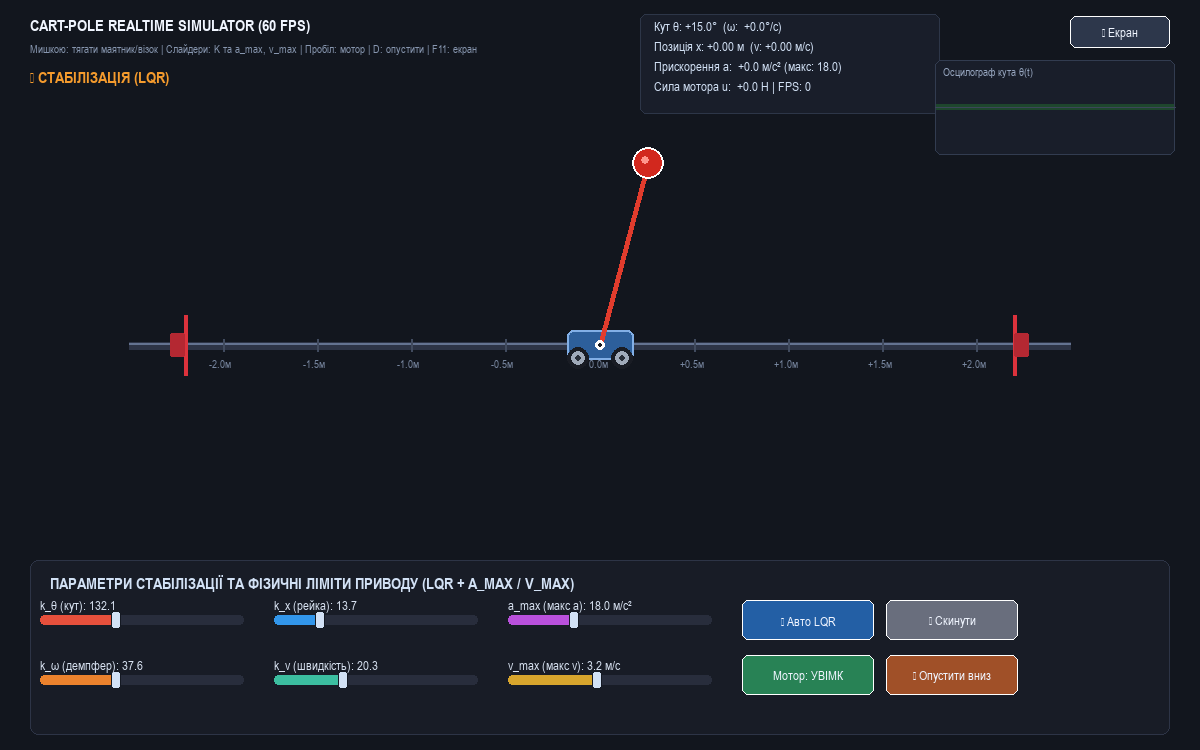
\includegraphics[width=0.92\columnwidth]{sim_pygame.png}
\caption{Real-time interactive 60~FPS simulation environment (\texttt{sim\_pygame.py}) displaying the inverted cart-pole, telemetry panel, interactive tuning sliders, and live oscilloscope.}
\label{fig:pygame}
\end{figure}

\subsection{Trajectory and Multi-Body Diagnostics}
Simulation diagnostics evaluate transient response characteristics. Fig.~\ref{fig:results} illustrates the closed-loop time-domain trajectory from the offline NMPC simulation (\texttt{dip\_results.png}), depicting the coordinated swing-up transition of both links into the vertical configuration alongside cart displacement and control force histories.

\begin{figure}[htbp]
\centering
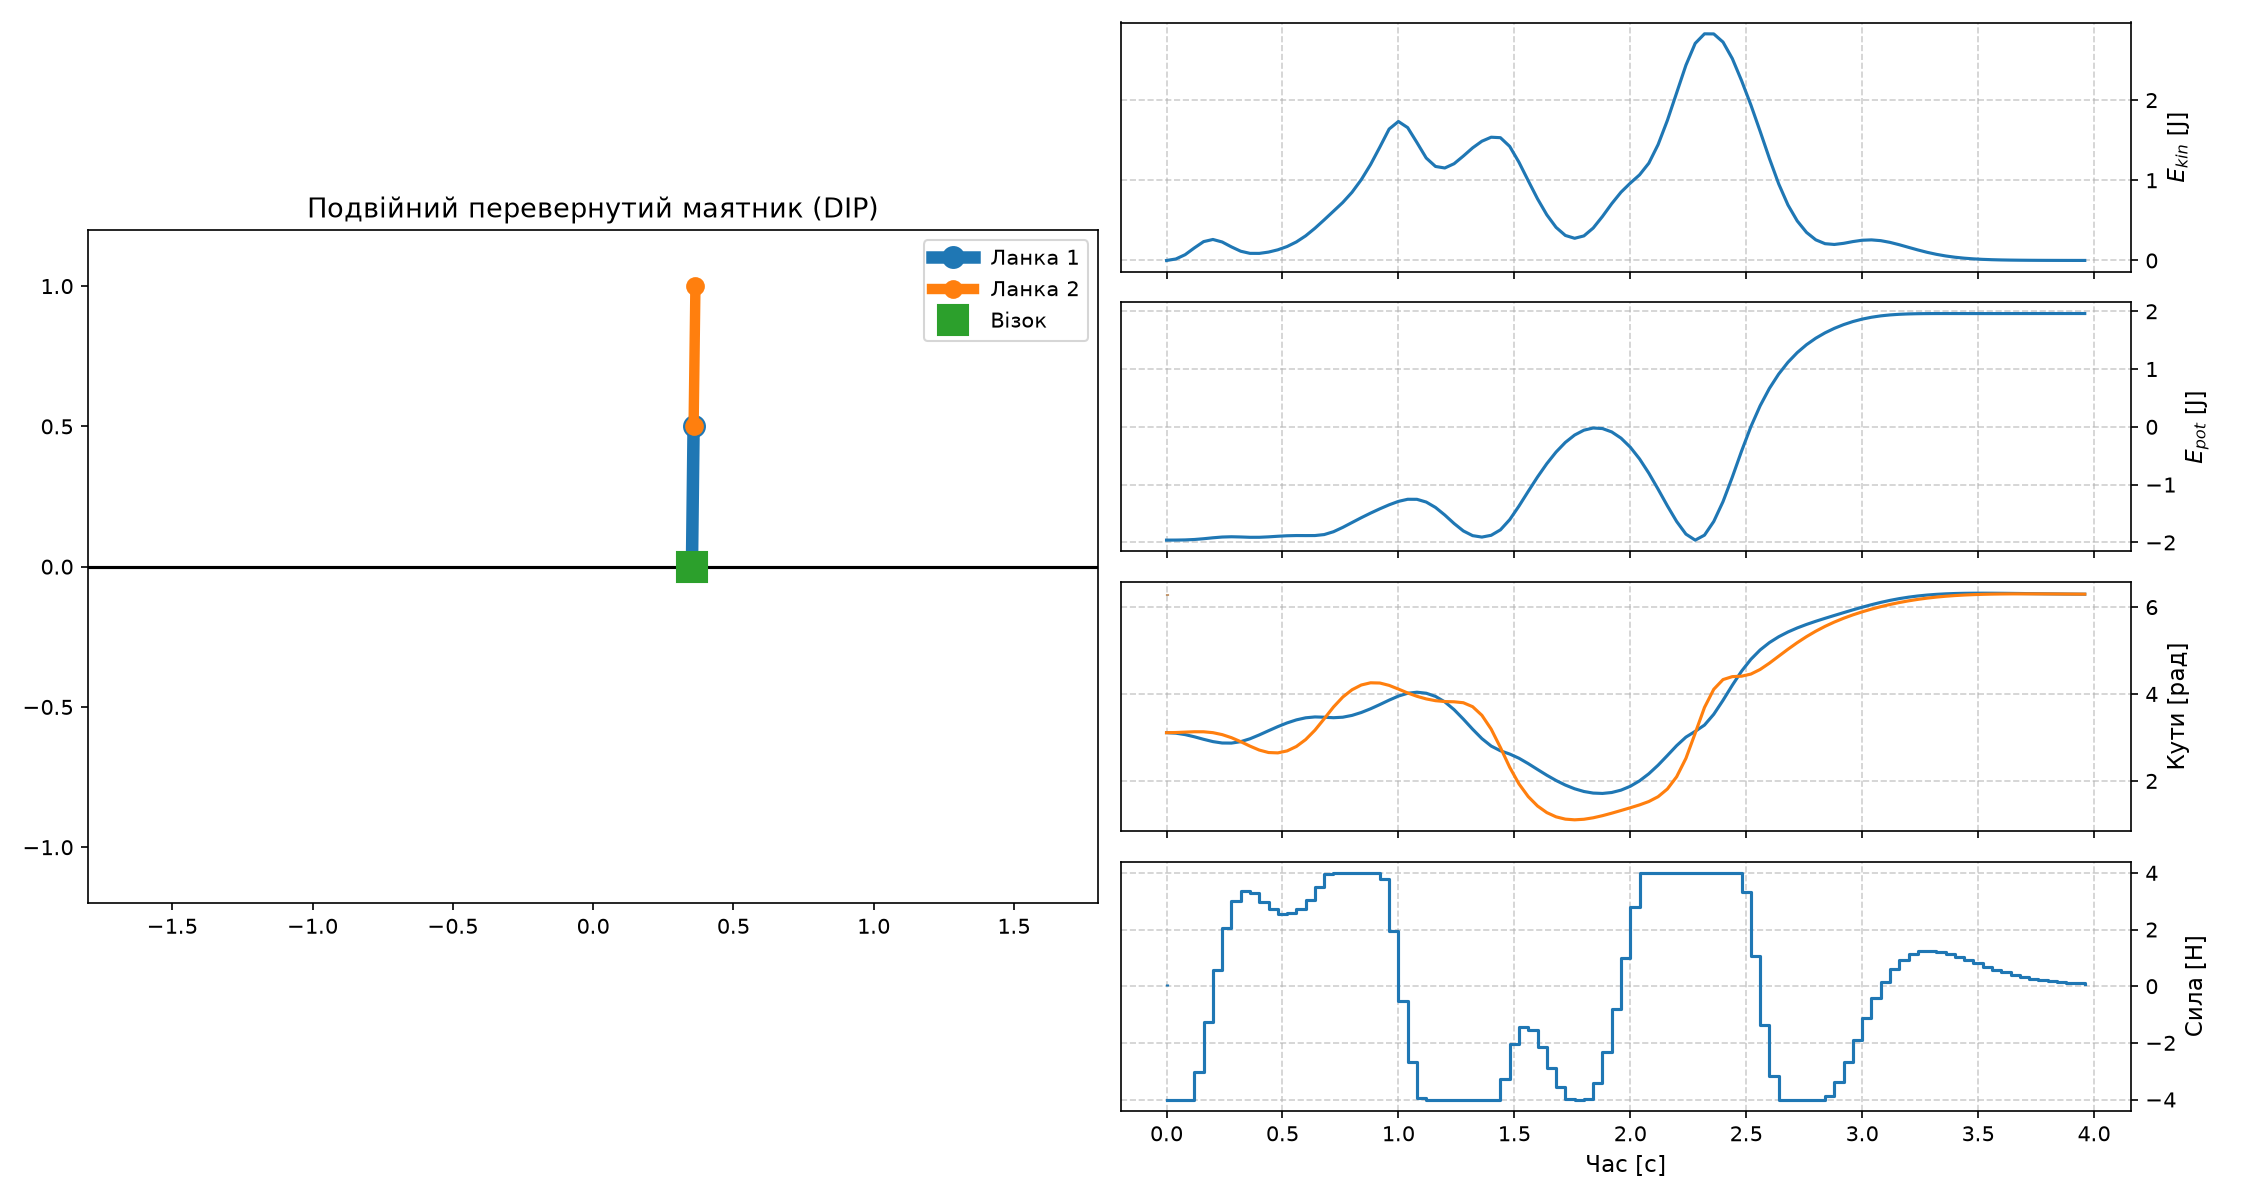
\includegraphics[width=0.98\columnwidth]{dip_results.png}
\caption{Time-domain trajectory results from \texttt{dip\_results.png} illustrating kinetic/potential energies, pendulum angles $\theta_1(t), \theta_2(t)$, and control force $u(t)$ during NMPC swing-up.}
\label{fig:results}
\end{figure}

\begin{figure}[htbp]
\centering
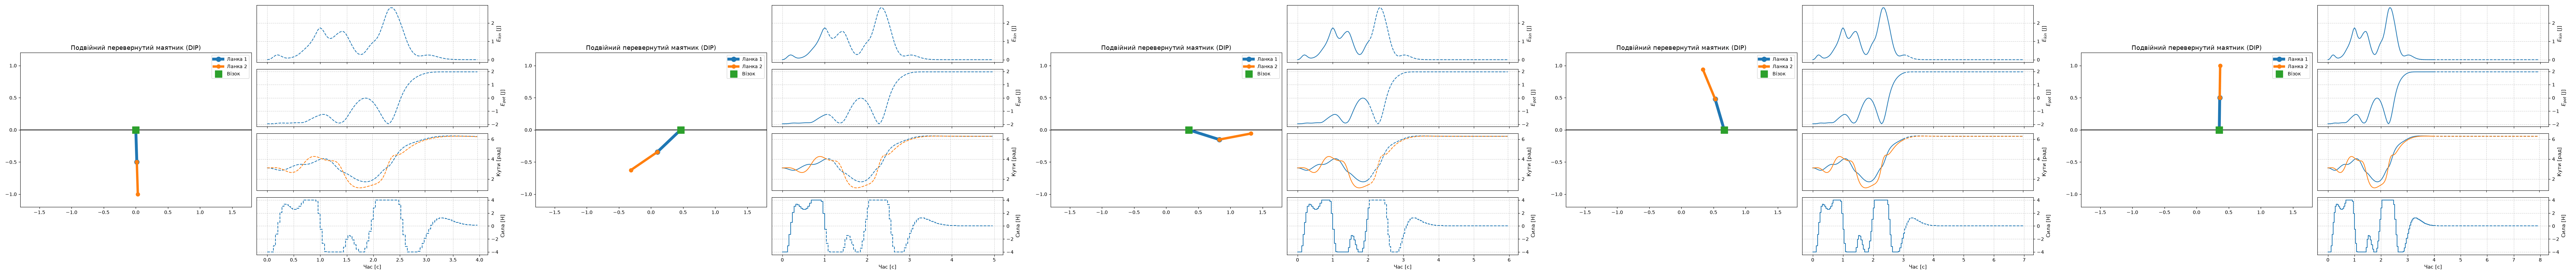
\includegraphics[width=0.95\columnwidth]{anim_dip.png}
\caption{Multi-body configuration sequence extracted from \texttt{anim\_dip.gif} illustrating the dynamic swing-up trajectory of the double inverted pendulum under optimal control.}
\label{fig:mpc_anim}
\end{figure}

\section{Embedded Microcontroller Implementation}

\subsection{Discrete Real-Time Control Loop}
To support direct deployment to embedded microcontrollers (e.g., STM32, ESP32), the LQR balancing law is formulated as a deterministic fixed-rate discrete routine. Listing~1 shows the implementation.

\begin{lstlisting}[language=C, caption={Embedded C/C++ control routine for real-time stabilization.}]
// Stabilization gains computed via CARE
const float K_THETA = 107.63f;
const float K_OMEGA = 30.74f;
const float K_X     = 10.00f;
const float K_V     = 15.73f;
const float MAX_FORCE = 19.80f; // Actuator limit

float x_pos = 0.0f;
float prev_theta = 0.0f;

void control_loop(float dt) {
    // 1. Read hardware sensors / encoders
    float theta = read_pendulum_angle_rad();
    float v     = read_cart_velocity_mps();

    // 2. Compute angular velocity & position
    float omega = (theta - prev_theta) / dt;
    x_pos += v * dt;
    prev_theta = theta;

    // 3. Evaluate state feedback control law
    float u = K_THETA * theta + K_OMEGA * omega
            + K_X * x_pos + K_V * v;

    // 4. Actuator saturation clamping
    if (u > MAX_FORCE)  u = MAX_FORCE;
    if (u < -MAX_FORCE) u = -MAX_FORCE;

    // 5. Output signal to motor driver (PWM+DIR)
    set_motor_output(u);
}
\end{lstlisting}

\subsection{Telemetry and Signal Conditioning}
On physical testbenches, optical quadrature encoders with resolutions up to 10,000 Counts Per Revolution (CPR) yield angular precision of $0.036^\circ$, critical for double pendulum balance. At a 500~Hz loop frequency ($\Delta t = 2$~ms), finite-difference velocity estimates $\omega_k \approx (\theta_k - \theta_{k-1})/\Delta t$ are processed through a discrete 1st-order low-pass filter ($f_c = 40$~Hz) to attenuate high-frequency encoder quantization noise prior to gain multiplication.

\section{Results and Performance Analysis}

\subsection{Disturbance Rejection Testing}
The dynamic robustness of the synthesized LQR controller was evaluated under simulated impulse perturbations. Applying an external horizontal disturbance of 15~N for 100~ms produces an instantaneous angular deflection of $4.8^\circ$. The controller accelerates the cart by 0.18~m beneath the falling center of mass, restoring verticality and centering the cart at $x = 0$ within 1.35~s without rail derailment.

\subsection{Architectural Comparison: LQR vs. NMPC}
Table~\ref{tab:comparison} contrasts the operational profiles of the local LQR stabilizer and the trajectory-optimizing NMPC controller.

\begin{table}[htbp]
\caption{Controller Characteristics Comparison: LQR vs. NMPC}
\begin{center}
\begin{tabular}{lcc}
\toprule
\textbf{Metric / Feature} & \textbf{LQR Balancing} & \textbf{NMPC Optimization} \\
\midrule
Execution model          & Real-time closed-loop   & Trajectory optimization \\
Computational cost       & $< 0.02$~ms per step    & $\approx 10$--$20$~ms (IPOPT) \\
Basin of attraction      & Local ($|\theta| < 28^\circ$) & Global ($|\theta| \le 180^\circ$) \\
Constraint handling      & Post-hoc clamping       & Explicit DAE bounds \\
Primary application      & Upright stabilization   & Energy-optimal swing-up \\
Target hardware          & Cortex-M4 / ESP32       & Linux SBC / PC workstation \\
\bottomrule
\end{tabular}
\label{tab:comparison}
\end{center}
\end{table}

While LQR requires minimal compute resources ($< 20~\mu$s), enabling execution on low-cost microcontrollers, it is constrained to a local operating basin. Conversely, NMPC optimizes non-convex trajectories over large state excursions, functioning as an optimal feedforward generator that handshakes with LQR upon vertical arrival.

\section{Conclusion and Future Work}
This paper presented an end-to-end modeling, simulation, and optimal control framework for underactuated single and double inverted pendulum systems on a linear motorized cart. Full nonlinear equations of motion were derived via Euler-Lagrange mechanics and validated using a 60~FPS Runge-Kutta simulator. The control architecture integrates Lyapunov energy pumping and NMPC trajectory generation for automated swing-up, coupled with LQR state-feedback for upright balance. The algorithms were translated into discrete C/C++ firmware ready for physical deployment.

Future work will focus on experimental validation using linear synchronous motor testbenches, real-time closed-loop NMPC using acados/qpOASES, and extending the multi-link formulation to triple inverted pendulums.

\section*{Acknowledgment}
The authors express sincere gratitude to project mentor Ivan Shevtsov (Staff Embedded Engineer, Samsung R\&D Institute Ukraine) for technical guidance. We also thank the Faculty of Applied Sciences of Ukrainian Catholic University for academic resources, and the Armed Forces of Ukraine for providing the security that makes this research possible.

\begin{thebibliography}{07}
\bibitem{ref_task} Faculty of Applied Sciences, Ukrainian Catholic University, ``Stabilization of Double/Triple Inverted Pendulum (ROBO:EN),'' Course Project Specification, 2024.
\bibitem{ref_git} T. Omelianchuk, S. Konoval, O. Oksentiuk, and O. Arlamovska, ``Double Pendulum Stabilization: Simulation and Control Repository,'' GitHub repository, 2024. [Online]. Available: https://github.com/timlim24/double-pendulum-stabilization
\bibitem{ref_spong} M. W. Spong, ``The swing up control problem for the Acrobot,'' \textit{IEEE Control Systems Magazine}, vol. 15, no. 1, pp. 49--55, Feb. 1995.
\bibitem{ref_astrom} K. J. \r{A}str\"{o}m and K. Furuta, ``Swinging up a pendulum by energy control,'' \textit{Automatica}, vol. 36, no. 2, pp. 287--295, 2000.
\bibitem{ref_brunton} S. L. Brunton and J. N. Kutz, \textit{Data-Driven Science and Engineering: Machine Learning, Dynamical Systems, and Control}, Cambridge University Press, 2019.
\bibitem{ref_casadi} J. A. Andersson, J. \r{A}kesson, and M. Diehl, ``CasADi: a software framework for nonlinear optimization and optimal control,'' \textit{Mathematical Programming Computation}, vol. 11, no. 1, pp. 1--36, 2019.
\bibitem{ref_den} K. Den et al., ``Design and control of a high-precision multi-armed pendulum cart benchmark system,'' in \textit{Proc. IEEE/RSJ Int. Conf. Intelligent Robots and Systems (IROS)}, 2023.
\end{thebibliography}

\end{document}
